\section{Tesztelés}

Az alábbi felsorolások a szoftver aktuális állapotának futó verzióján általam
kipróbált műveleteket és azok eredményeit tartalmazzák, funkciók szerint
csoportosítva.

\subsection{Hőtérképes megjelenítés}

\begin{itemize}

  \item Egy hőtérkép réteg létrehozása után a feliratkozások beállítását
  követően azonnal elkezdtek megjelenni a mérési pontok a térképen

  \item A színezési függvény, az értékhatárok és a színtartomány bármelyikének
  átállítását követően az "UPDATE PARAMETERS" gomb a jelölők újrarajzolását
  eredményezte a módosított paraméterek tekintetében.

\end{itemize}


\subsection{Térkép állapotainak (pozíció, forgatás, nagyítás) tárolása és betöltése}

\begin{itemize}

  \item Az aktuális pozíció eltárolására szolgáló listaelemre kattintva megnyílt
  az adatainak szerkesztésére szolgáló dialógusablak, melyben a bejegyzés neve
  megadható, a mentés véglegesíthető vagy pedig megszakítható volt. A mentést
  választva a bejegyzés hozzáadódott a lista aljára.

  \item Egy elmentett pozícióhoz tartozó listaelemre kattintva a térkép
  betöltötte a hozzá tartozó állapotot.

  \item Egy elmentett pozíció listaeleme melletti fogaskerék ikonra kattintva
  megnyílt az annak szerkesztésére szolgáló dialógusablak, melyből
  módosíthatóak voltak a hozzá tartozó paraméterek, a végrehajtott módosítások
  elmenthetők vagy pedig elvethetők voltak, továbbá a teljes bejegyzés is
  törölhető volt.

\end{itemize}


\subsection{Objektumok betöltése GeoJSON formátumból}

\begin{itemize}

  \item Hibás tartalom esetén az "IMPORT GEOJSON" gomb megnyomását követően a
  képernyő alsó szélén egy felugró üzenet jelezte, hogy helytelen a GeoJSON
  adat. (Az üres mezőt kipróbálva az is hibás adatnak számított, hiszen a nulla
  hosszúságú sztring nem valid GeoJSON. A mező kezdeti értéke "\{\}".) A bevitt
  adat ekkor nem került rögzítésre, így a legutolsó valid tartalom maradt
  kirajzolva a térképre.

  \item Helyes tartalom esetén az import "IMPORT GEOJSON" gombra kattintva az
  adat által leírt objektumok megjelentek a térképen a beállított kitöltési és
  körvonalazási színekkel. Az előzőleg megjelenített objektumok pedig eltűntek.
  (Tehát több különálló adat kirajzolásához több GeoJSON réteg létrehozása
  szükséges.)

\end{itemize}


\subsection{Parancsok kiadása drónoknak menüsorról és jobb egérgombra felugró ablakból}

\begin{itemize}

  \item Amennyiben egy drón sem volt kijelölve, akkor a jobb klikk menüben és az
  eszköztárban is inaktívak (tehát szürkék és nem kattinthatóak) voltak a
  gombok.

  \item Legalább egy kijelölt drón esetén a gombok aktívvá váltak.

  \item Egy parancshoz tartozó gombra történő kattintás után a drónok
  végrehajtották a kapott parancsot (a teszt szerver által szimulált drónok csak
  a leszállás és felszállás parancsok végrehajtását támogatják), az
  eseménynaplóba pedig bejegyzés került, amikor visszajelzés érkezett a
  szervertől, hogy megérkezett hozzá az utasítás kiadását kezdeményező üzenet.

\end{itemize}


\subsection{Állapotüzenetek (információk, figyelmeztetések, hibák) kijelzésére alkalmas panel}

\begin{itemize}

  \item Új állapotüzenet érkezésekor a táblázat megjelenítette a bejegyzést.

\end{itemize}


\subsection{Drónok színkódolása predikátumok alapján}

\begin{itemize}

  \item Üresen hagyott mező esetén a szín egyik drónra sem érvényesült.

  \item Helyesen kitöltött mező esetén az "APPLY CHANGES" gomb (vagy az Enter
  billentyű) megnyomása után a szín azokra a feltételt teljesítő drónokra
  érvényesült, amelyeket nem írt felül más predikátumok teljesülése.

  \item Hibásan kitöltött mező esetén az "APPLY CHANGES" gomb (vagy az Enter
  billentyű) megnyomását követően a hibás mező címkéje és alsó szegélye piros
  színűre váltott, a hiba szövege pedig bekerült az eseménynaplóba. A bevitt
  érték nem került rögzítésre, tehát a szín azokra a drónokra maradt érvényes,
  amelyek a mező által előzőleg tartalmazott legutolsó valid predikátumot
  teljesítették.

\end{itemize}


\subsection{Drónok részletes aktuális állapotát mutató panel}

\begin{itemize}

  \item A táblázat helyesen kijelezte a drónokról jelenleg ismert információkat.

\end{itemize}


\subsection{Kliens állomás pozíciójának megjelenítése a térképen geolokáció alapján}

\begin{itemize}

  \item Ha nem volt elérhető pozícióra vonatkozó adat (például asztali
  böngészőben letiltva a geolokációt, illetve mobiltelefonon kikapcsolva a
  GPS-t), akkor a jelölő nem került rá a térképre és az eseménynaplóban
  megjelent egy erre vonatkozó bejegyzés.
  \begin{figure}[H]
    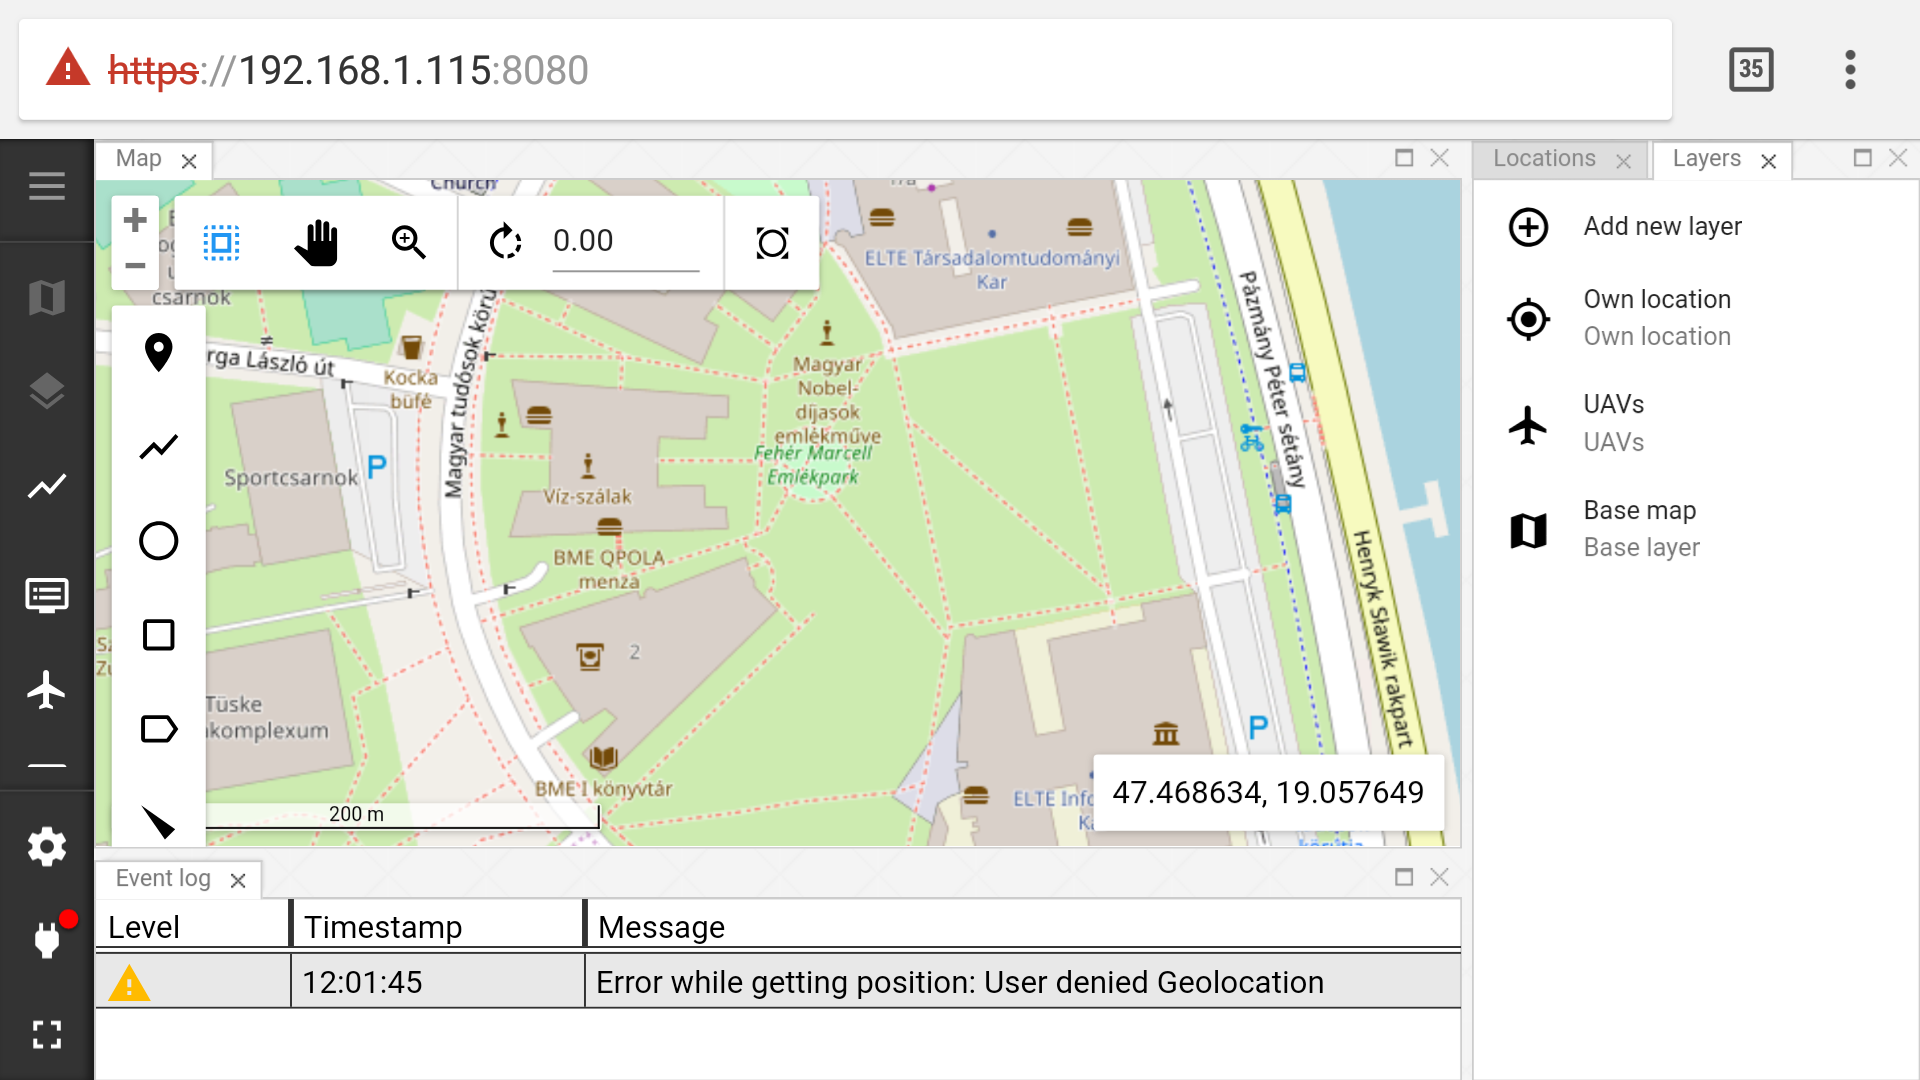
\includegraphics[width=\textwidth]{phone_gps_denied.png}
    \caption{Mobil eszköz kikapcsolt GPS-el}
    \label{fig:phone_gps_denied}
  \end{figure}

  \item Ha elérhető volt a geolokáció szolgáltatás, akkor a jelölő felkerült a
  térkép megfelelő pontjára, valamint a pozíció megváltozásakor frissült és
  követte az elmozdulást.

  \item Ha mágneses orientációérzékelő is elérhető volt az eszközben
  (mobiltelefonon tesztelve), akkor a jelölő követte annak elfordulását.
  (Ez a funkció már előzőleg működőképes volt, azonban hosszú időn át nem került
  sor az ellenőrzésére abból az okból, hogy mágneses érzékelő általában csak
  mobiltelefonokban van. Laptopról legfeljebb csak emulálni lehet, a telefonról
  történő teszteléshez pedig publikus https szerver indítása szükséges, mert a
  geolokációhoz csak titkosított (vagy megbízható, például "localhost")
  kapcsolat esetén biztosítanak hozzáférést a modern böngészők. Ebből adódott,
  hogy csak most, miután tesztelés közben nem működött, derült fény arra, hogy
  az eredeti megvalósításához használt, OpenLayers könyvtárból származó
  DeviceOrientation osztály a legutóbbi verzióban már elavultnak lett
  nyilvánítva és a tapasztalat alapján nem is funkcionál rendesen. Áttérve a
  közvetlenül a böngésző által rendelkezésre bocsátott "deviceorientation"
  esemény figyelésére újra működésbe lépett a funkció, mint az a képen
  (\ref{fig:phone_compass}. ábra) is látható.)

  \begin{figure}[H]
    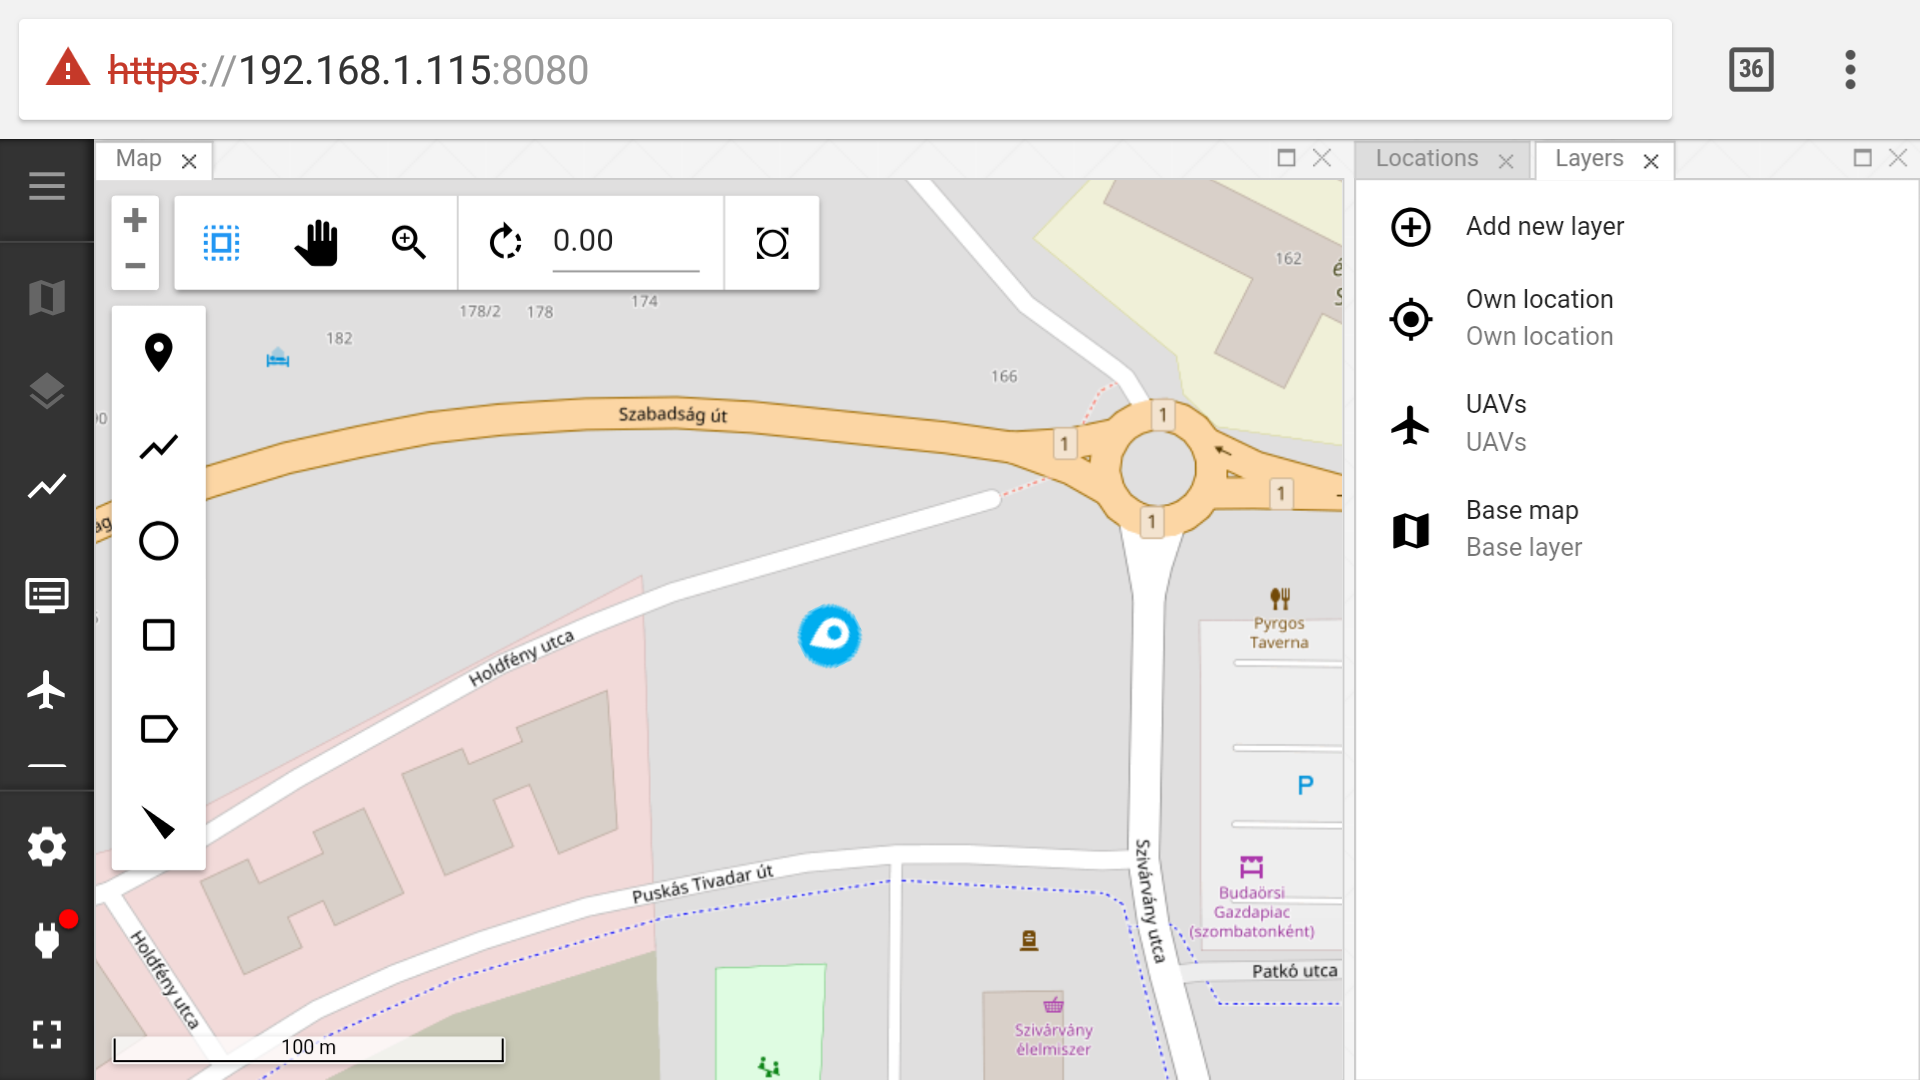
\includegraphics[width=\textwidth]{phone_compass.png}
    \caption{Iránytű alapján elforduló jelölő mobil eszközön}
    \label{fig:phone_compass}
  \end{figure}

\end{itemize}


\subsection{Billentyűkombinációkkal történő vezérlés}

\begin{itemize}

  \item Minden billentyűkombináció megfelelően működött.

\end{itemize}


\subsection{Nagy számú drón kezelése}

Hatékonyság szempontjából a felület tesztelésre került különböző számú szimulált
drónnal, változatos üzenetsűrűségekkel. A tapasztalat az, hogy 40 kopter esetén
nagyjából (drónonként) 0.3 másodpercenként érkező üzenetek esetén éri el az
alkalmazás aktív használat közben egy 2.5GHz-es órajelen üzemelő processzormag
kapacitásának határait. Ekkor a felület még használható marad, de már elkezdenek
szaggatni az animációk. Ezek alapján a szoftver bár képes a kitűzött cél
ellátására, azért a felhasználói élmény javításának érdekében még további
optimalizációra szorul a későbbiekben.
